\subsection{Implementation}
The implementation phase should follow the \hyperref[fig:eMSP-component]{component diagram}. \ac{eMall} and the \ac{CPMS} could be implemented at the same time by different teams. The two components are fully independent and if the interfaces are respected the development of one should not interfere with the other. This is permitted thanks to the usage of the bridge pattern (see \autoref{pattern:bridge}).\\
In this section \ac{eMall} and \ac{CPMS} will be analyzed separately following a bottom up strategy.\\
External components (\ac{API}) are considered already finished and tested, furthermore they will not be discussed in this section.
\subsubsection{eMall}
The implementation should be divided in 3 layers to be developed in the following order
\begin{enumerate}
    \item Model: The eMallModel should be the first component to be developed being the core of the system. The divide and conquer pattern should be used as much as possible to allow the whole team to work at the same time.
    \item Middle components: the second wave of development should focus on the: \ac{CPMS}\ac{API}, AuthenticationComponent, Payment\ac{API} and Mail\ac{API}. This components are independent from each other and should be developed at the same time compatibly with the team size.
    \item Leaf components: finally the last components can be implemented at the same time compatibly with the team size.
\end{enumerate}
Once the logic of the system is completed the apps (eMallClient: the view in \ac{MVC} pattern) (for users and \acp{CPO}) should be developed.
\subsubsection{CPMS}
Similarly to the \ac{eMall} the \ac{CPMS} should be implemented in 3 parts
\begin{enumerate}
    \item Model: The CPMSModel should be the first component to be developed being the core of the system. The divide and conquer pattern should be used as much as possible to allow the whole team to work at the same time.
    \item Middle components: the second wave of development should focus on the: CPMSAuthenticationComponent, CPMSChargingStation\ac{API}. This components are independent from each others and should be developed at the same time compatibly with the team size.
    \item Leaf components: finally the last components can be implemented at the same time compatibly with the team size.
\end{enumerate}
Once the logic of the system is completed the website (for \ac{CPO}Maintainers) should be developed.
\subsection{Integration and Test Plan}
The components should be integrated and unit tested. Each component inside the same layer can be tested autonomously giving the single teams the flexibility needed to solve problems that arose during testing. The unit testing shall be done using a driver to simulate the rest of the system.
The single units of the same abstraction level are fully testable independently, thus a parallel integration and test campaign can be sustained depending on the team's flexibility. A white box testing for each unit is mandatory to cover as much code and branches as possible. A good level of path coverage is above 80\%. At the end of the unit tests a series of black box tests must be done to confirm that the system behaves like expected. \cite{ref:box-testing}
\subsubsection{eMall}
\begin{figure}[H]
    \centering
    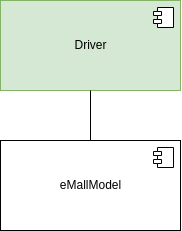
\includegraphics[keepaspectratio]{Testing/emall/emallModel.drawio.png}
    \caption{\ac{eMall} model testing}
\end{figure}
\begin{figure}[H]
    \centering
    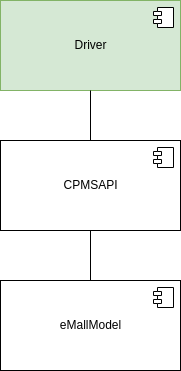
\includegraphics[keepaspectratio]{Testing/emall/cpmsapi.png}
    \caption{\ac{CPMS}\ac{API} testing}
\end{figure}
\begin{figure}[H]
    \centering
    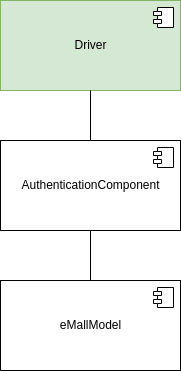
\includegraphics[keepaspectratio]{Testing/emall/authentication.drawio.png}
    \caption{AuthenticationComponent testing}
\end{figure}
\begin{figure}[H]
    \centering
    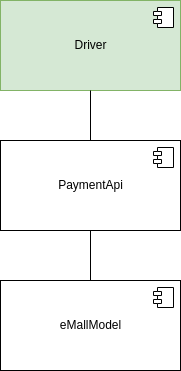
\includegraphics[keepaspectratio]{Testing/emall/payment.png}
    \caption{Payment \ac{API} testing}
\end{figure}
\begin{figure}[H]
    \centering
    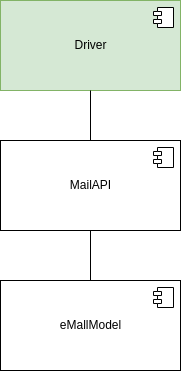
\includegraphics[keepaspectratio]{Testing/emall/mail.png}
    \caption{Mail\ac{API} testing}
\end{figure}
\begin{figure}[H]
    \centering
    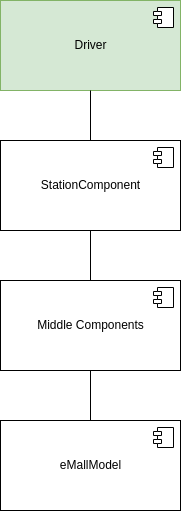
\includegraphics[keepaspectratio]{Testing/emall/station.png}
    \caption{StationComponent testing}
\end{figure}
\begin{figure}[H]
    \centering
    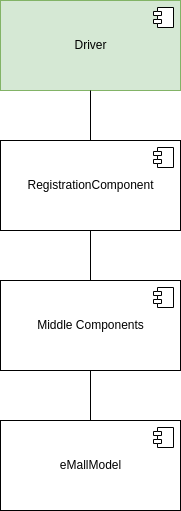
\includegraphics[keepaspectratio]{Testing/emall/registration.png}
    \caption{RegistrationComponent testing}
\end{figure}
\begin{figure}[H]
    \centering
    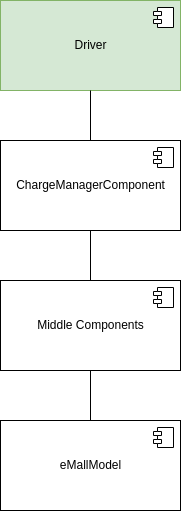
\includegraphics[keepaspectratio]{Testing/emall/chargemanager.png}
    \caption{ChargeManagerComponent testing}
\end{figure}
\begin{figure}[H]
    \centering
    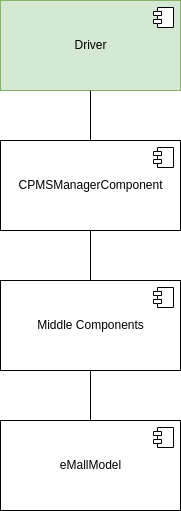
\includegraphics[keepaspectratio]{Testing/emall/cpmsmanager.png}
    \caption{\ac{CPMS}ManagerComponent testing}
\end{figure}
\begin{figure}[H]
    \centering
    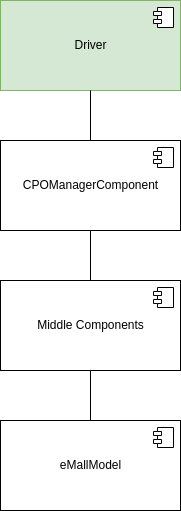
\includegraphics[keepaspectratio]{Testing/emall/cpomanager.png}
    \caption{\ac{CPO}ManagerComponent testing}
\end{figure}
\begin{figure}[H]
    \centering
    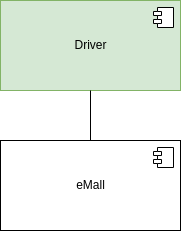
\includegraphics[keepaspectratio]{Testing/emall/emall.png}
    \caption{\ac{eMall} testing}
\end{figure}
\subsubsection{CPMS}

\begin{figure}[H]
    \centering
    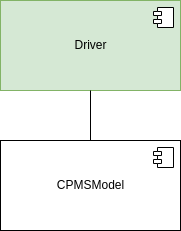
\includegraphics[keepaspectratio]{Testing/CPMS/cpms-CPMSModel.drawio.png}
    \caption{\ac{CPMS}Model testing}
\end{figure}
\begin{figure}[H]
    \centering
    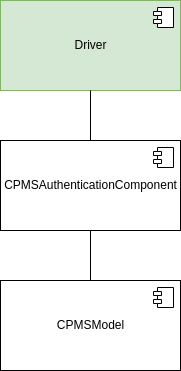
\includegraphics[keepaspectratio]{Testing/CPMS/cpms-CPMSAuthenticationComponent.drawio.png}
    \caption{\ac{CPMS}AuthenticationComponent testing}
\end{figure}
\begin{figure}[H]
    \centering
    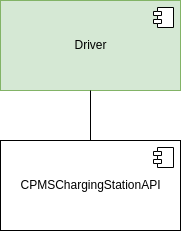
\includegraphics[keepaspectratio]{Testing/CPMS/cpms-CPMSCharging.drawio.png}
    \caption{\ac{CPMS}ChargingStation testing}
\end{figure}
\begin{figure}[H]
    \centering
    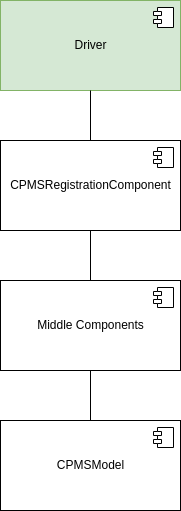
\includegraphics[keepaspectratio]{Testing/CPMS/cpms-CPMSRegistration.drawio.png}
    \caption{\ac{CPMS}RegistrationComponent testing}
\end{figure}
\begin{figure}[H]
    \centering
    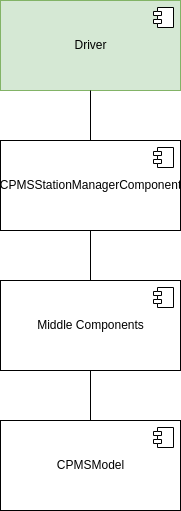
\includegraphics[keepaspectratio]{Testing/CPMS/cpms-CPMSStationManager.drawio.png}
    \caption{\ac{CPMS}StationManagerComponent testing}
\end{figure}
\begin{figure}[H]
    \centering
    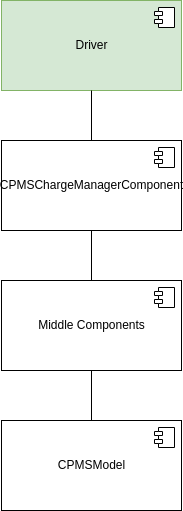
\includegraphics[keepaspectratio]{Testing/CPMS/cpms-CPMSChargeManagerComponent.drawio.png}
    \caption{\ac{CPMS}ChargeManagerComponent testing}
\end{figure}
\begin{figure}[H]
    \centering
    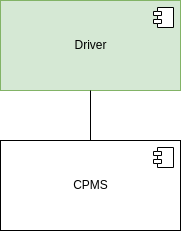
\includegraphics[keepaspectratio]{Testing/CPMS/cpms-CPMS.drawio.png}
    \caption{\ac{CPMS} testing}
\end{figure}

\clearpage